\documentclass[11pt]{amsart}
\usepackage{geometry}                % See geometry.pdf to learn the layout options. There are lots.
\geometry{letterpaper}                   % ... or a4paper or a5paper or ...
%\geometry{landscape}                % Activate for for rotated page geometry
%\usepackage[parfill]{parskip}    % Activate to begin paragraphs with an empty line rather than an indent
\usepackage{booktabs}
\usepackage{graphicx}
\usepackage{amssymb}
\usepackage{epstopdf}
\usepackage{caption}
\usepackage{subcaption}
\usepackage{commath}
\DeclareGraphicsRule{.tif}{png}{.png}{`convert #1 `dirname #1`/`basename #1 .tif`.png}

% Declare commands
\newcommand{\mat}[1]{\mathbf{#1}}
\DeclareMathOperator*{\argmax}{arg\,max}

\title{CS 181 -- Practical 4}
\author{Casey Grun, Sam Kim, Rhed Shi}
%\date{}                                           % Activate to display a given date or no date

\begin{document}
\maketitle

% -----------------------------------------------------------------------------
\section{Warmup}

The method to attack this problem is not necessarily straightforward at first sight, because on one hand, the game definitively ends when the score is 101 or higher, and on the other hand, it is possible to have an infinitely long game if one constantly misses their target and hits a blank space. Because of this latter possibility, we used an infinite horizon model to solve the game. Additionally, we implemented the policy learning algorithm as opposed to the value learning algorithm because the policy algorithm is generally considered to be better in practice.

Most of the algorithm for policy iteration is straightforward, as we can solve for the best policy given the transition probabilities and values of each state using the Bellman equations
$$\pi^*(s)=\text{argmax}_{a\in A}\left[R(s,a)+\gamma\sum_{s'\in S} P(s'|s,a)V^*(s')\right]$$
and when $\pi^*(s)$ remains constant in successive iterations, we have reached the optimal policy. $P(s'|s,a)$, the transition probabilities, are given by the problem. The trick is how to calculate $V^*(s')$. The values satisfy
$$V^*(s)=R(s,\pi^*(s))+\gamma\sum_{s'\in S} P(s'|s,\pi^*(s))V^*(s')$$
which has a unique solution.

To solve this, we set $V(101)=1$ and $V(i)=-1$ for $i \in \{102,103,...,117\}$, because after reaching these states, the game ends, so these are the final values. In this formulation, $R=0$ for all states. Plugging these into the above equation and rearranging, we get
$$\sum_{s'=0}^{100} P(s'|s,\pi^*(s))V^*(s) - \frac{1}{\gamma}V^*(s')=-P(100|s,\pi^*(s))+\sum_{s'=102}^{117} P(s'|s,\pi^*(s))V^*(s')$$

This can be expressed as a matrix equation $Ax=b$ where $x=V^*(s)$, which is easily solvable given that $A$ is invertible. The final values as a function of the state are shown in the figure below. $\gamma=1$.

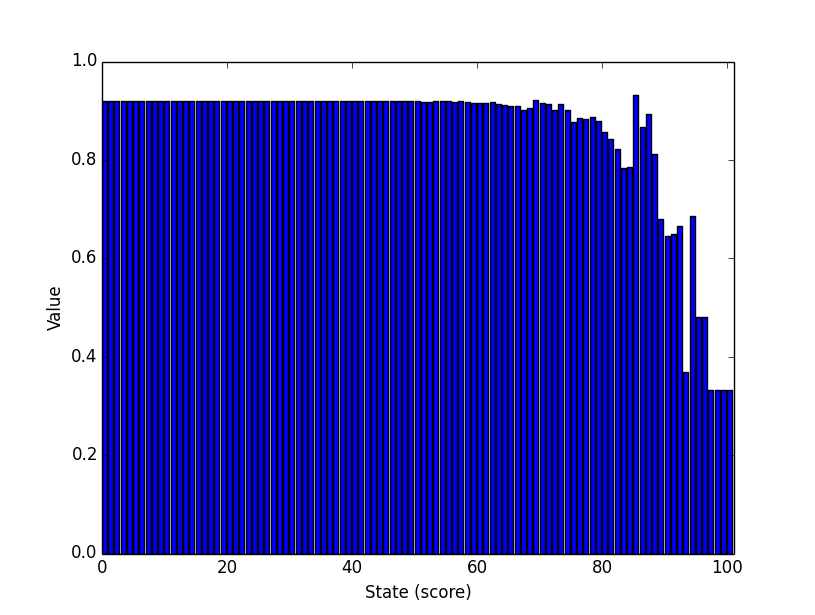
\includegraphics[width=14cm]{values_gamma1.png}

We can see a peak at the state $s=85$, which is 16 below the winning score of $101$. The peak occurs here because in addition to having a $60\%$ chance of hitting the 16 on the dart board, if it misses, there is still a chance to reach 101 because the score has not gone over. For subsequent states, the value drops because there is a chance of going over if one misses the target, especially as the state approaches 101. 
The states below 85 show a similar structure in which the states closer to 0 have a high value, and it steadily decreases as the state approaches 85. This is because for the states right below 85, it is likely to reach a state between 85 and 101, which are not optimal. We can think of the state $s=85$ as a secondary target.

% -----------------------------------------------------------------------------
\section{Reinforcement Learning}

Our challenge for this week was to implement a reinforcement learning to play
the game ``Swingy Monkey.'' We pursued three independent approaches to solve this 
problem:

\subsection{Q-learning}

First, we implemented a the model-free ``Q-learning'' algorithm. Q-learning works
by learning the function $Q(s,a)$ (the expected value of an action $a$ from a 
state $s$). We begin with a uniform estimate of $Q(s,a) = 0 \forall s \forall a$.
At each time point during epoch $t$, we plan the next action $\pi(s)$ given the 
current state $s$, according to the following ``$\epsilon$-greedy'' policy:
$$\pi_t(s) = \begin{cases} 
\argmax_{a \in \mathcal{A}} Q(s,a) & \text{with probability } 1-\epsilon(t) \\
\text{random } a \in {0,1}         & \text{with probability } \epsilon(t) 
\end{cases}$$
where $\epsilon(t) = 1/t$. This allows exploration of new states at early time 
points and exploitation at later time points.

Upon taking an action $a$ (during epoch $t$), recieving a reward $r$, and observing a transition from $s$
to $s'$, we update our running estimate of $Q(s,a)$ as follows:
$$Q(s,a) \gets Q(s,a) + \alpha_k(s,a) \left[ (r + \gamma \max_{a' \in \mathcal{A}} Q(s', a')) - Q(s,a) \right].$$
We attempted a strategy where the learning rate $\alpha_k(s,a) = 1/k$, and $k$ is the number of times we've visited state $s$ and performed action $a$. This reflects our desire to gradually reduce the rate of change of our 
policy (and therefore $Q$) over epochs in order to exploit the benefits of our earlier exploration. However, we had much poorer results with this strategy than one where we simply set $\alpha_k(s,a) = 0.1 \forall(s,a,k)$.

\subsection{Model-based learning}

\subsection{TD-value learning}

Finally, we implemented temporal difference value learning. In this method, we learn a model of the value function $V(s)$, the transition model $P(s'|s,a)$, and the reward function $R(s,a)$. The transition model was learned as in the model-based approach above, where we maintained the empirical distribution. The reward function was learned by a running average, where each time we recieved a reward $r$ from taking action $a$ at state $s$ for the $k$-th time, we updated $R(s,a)$ as:
$$R(s,a) \gets (R(s,a) * k + r)/(k + 1).$$

Each time we transitioned to state $s'$ from state $s$ and received reward $r$, we updated the value function according to:
$$V(s) \gets V(s) + \alpha ((r + \gamma V(s')) - V(s)).$$
At each step, we planned the next action $\pi(s)$ according to:
$$\pi(s) = \argmax_{a \in \mathcal{A}} \left[ R(s,a) + \sum_{s'} P(s'|s,a) V(s') \right]$$
where $R(s,a)$, $P(s'|s,a)$, and $V(s)$ represent our empirically-estimated values for those quantities.

% -----------------------------------------------------------------------------
\section{Conclusion}


% -----------------------------------------------------------------------------
\begingroup
\begin{thebibliography}{9}

%\bibitem{LSMR}
%Fong, David Chin-Lung, and Michael Saunders. "LSMR: An iterative algorithm for sparse least-squares problems."
%\emph{SIAM Journal on Scientific Computing} 33.5 (2011): 2950-2971

\end{thebibliography}
\endgroup

\end{document}